\documentclass[openany]{memoir}
\usepackage{amsmath, amsfonts, amsthm}
\usepackage{lipsum}
\usepackage{algorithm, algorithmic}
\usepackage[english]{babel}
\usepackage[T1]{fontenc}
\usepackage{CJKutf8}
\newcommand\textkorean[1]{\begin{CJK}{UTF8}{mj}#1\end{CJK}}
\usepackage{graphicx}

\begin{document}

\title{Notes on Portfolios}
\author{JeaSung Park\\
Soongsil University, Seoul}
\date{15 January 2018}
\maketitle

\clearpage
\begin{abstract}
\textkorean{안녕하십니까? 컴퓨터비전을 활용해 인간에게 도움이 되는 좋은 소프트웨어를 만들고 싶은 박재성입니다. 병렬 처리를 통해 빠른 연산을 해내는 그래픽 처리 장치에 매료되어 이 분야에 첫 발을 내딛게 되었고, 확률 그래프 모델을 활용한 이미지 분석에 관심을 가지고 2 년간 공부하였습니다. 이 부서에 지원하게 된 까닭은 딥러닝 모델 설계의 자동화를 통해 기존 모델 대비 정확도가 향상된 모델을 만들고 싶어서이며, 해당 분야를 연구함에 있어 저의 기계학습 전반에 대한 이해와 그래프 모델을 응용한 접근이 도움이 될 것이라고 생각했기 때문입니다. 기술 본위의 IT 회사인 카카오에서 우수한 연구원분들과 함께 협업하며 좋은 결과를 이끌어내고 싶습니다. 감사합니다.}
\end{abstract}

\chapter{Covariance Selection}
\section{Sparse inverse covariance estimation with the graphical lasso}
Before explaining some of the important properties in multivariate statistical analaysis, I will introduce some notations for ease of reading.
\begin{description}
	\item[Definition] An \textit{exterior differential form} of degree $r$ in $\mathbb{R}^{m}$ is an expression of the type
	$$\sum_{t_1 < t_2 < \cdots < t_r} h_{t_1, \cdots, t_r}(x)dx_{t1} \land \cdots \land dx_{t_r}$$
	where the $h_{t_1, \cdots, t_r}$ are analytic functions of $x_1, \cdots, x_m$ \qed
\end{description}

This definition comes with an important property that is fundamental to changing variables from one to another.

\begin{description}
\item[Theorem] If $dy$ is an $m \times 1$ vector of differentials and if $dx=Bdy$, where $B$ is an $m \times m$ nonsingular matrix(so that $dx$ is a vector of linear differential forms), then
$$\bigwedge_{i=1}^{m} dx_i = detB \bigwedge_{i=1}^{m} dy_i$$ \qed
\end{description}

There is another notation I need to introduce. This is important because there is no other ways to express the sampling distribution of some distribution clearer than this.

\begin{description} 
	\item[Definition] Let $A=(a_{i,j})$ be a $p \times q$ matrix and $B=(b_{i,j})$ be an $r \times s$ matrix. The Kronecker product of A and B, denoted by $A \otimes B$, is the $pr \times qs$ matrix 
	$$A \otimes B = \begin{bmatrix}
	a_{11}B & a_{12}B & \cdots & a_{1q}B \\
	a_{11}B & a_{12}B & \cdots & a_{1q}B \\
	\vdots \\
    a_{p1}B & a_{p2}B & ... & a_{pq}B
    \end{bmatrix}$$ \qed
\end{description}

We now have notations sufficient for explaining a sampling distribution of mean and covariance. Define the mean and covariance as follows.
\begin{equation}
\begin{gathered}
$$\bar{X} = \frac{1}{N} \sum_{i=1}^{N} X_i \\
S = \frac{1}{n}A$$
\end{gathered}
\end{equation}
where $A = \sum_{i=1}^{N} (X_i - \bar{X})(X^{T}_{i} - \bar{X})^{T}$\\

Then, we can prove the following result.

\begin{description}
\item[Theorem] If the $N \times m$ matrix $X$ is $N(1\mu^{T}, I_N \otimes \Sigma)$ then $\bar{X}$ and $A$, defined by (1.1), are independently distributed; $\bar{X}$ is $N_m(\mu, \frac{1}{N} \Sigma)$ and $A$ has the same distribution as $Z^TZ$, where the $n \times m(n = N - 1)$ matrix $Z$ is $N(0, I_n \otimes \Sigma)$(i.e. the $n$ rows of $Z$ are independent $N_m(0^T, \Sigma)$ random vectors). \qed
\end{description}

Motivated by the above theorem, I now introduce a distribution called \textit{Wishart distribution}

\begin{description}
\item[Definition] If $A = Z^TZ$ where the $n \times m$ matrix $Z$ is $N(0, I_n \otimes \Sigma)$, then $A$ is said to have the \textit{Wishart distribution} with $n$ degrees of freedom and covariance $\Sigma$. We will write that $A$ is $W_m(n, \Sigma)$, the subscript on $W$ denoting the size of the matrix $A$. \qed
\end{description}

We now have the definition of Wishart distribution. This comes with a natural question on the probability density function of Wishart distribution. The following theorem gives the density function of $A$ when $n \geq m$.

\begin{description}
\item[Theorem] If $A$ is $W_m(n, \Sigma)$ with $n \geq m$ then the density function of $A$ is
$$\frac{1}{2^{mn / 2} \Gamma_m(\frac{1}{2}n)(det(\Sigma)^{n/2}} exp(tr(-\frac{1}{2}\Sigma^{-1}A))(detA)^{(n - m - 1) / 2}$$
where $\Gamma_m(\bullet)$ denotes the multivariate gamma function. \qed
\end{description}

Suppose we want to estimate the covariance matrix given a data normally distributed. Then the sampling distribution will surely follow the Wishart distribution and as such, finding a maximum likelihood solution gives the desired result. So we propose an objective function below and try to find its global maximum(or minimum vice versa).

\begin{equation}
\begin{gathered}
$$l_1(\Sigma, \phi) = tr(\Sigma^{-1}\phi) - logdet(\Sigma^{-1} \phi) - m$$
\end{gathered}
\end{equation}
where $\phi = \hat{\Sigma}$ is a sampled estimate of the true covariance matrix.

If we restrict the solution space of the problem above, we can prove that the best solution is an unbiased estimate of the covariance matrix.

\begin{description}
\item[Theorem] Using the loss function $l_1(\Sigma, \phi)$, the best(smallest risk) estimate of $\Sigma$ having the form $\alpha A$ is the unibiased estimate $S = \frac{1}{n}A$. \qed
\end{description}

 The thing is that we can do better than the sample covariance matrix $S$ if we look outside the class of estimates of the form $\alpha A$. James and Stein(1961) have shown using an \textit{invariance argument} to prove this result. It is reasonable to require that if $\phi(A)$ estimates $\Sigma$ and $L$ is a nonsingular $m \times m$ matrix, then $\phi$ should satisfy
 $$\phi(L^TAL) = L^T\phi(A)L$$
 for $L^TAL$ is $W_m(n, L^T\Sigma L)$, so that $\phi(L^TAL)$ estimates $L^T\Sigma L$. Then 
 
 \begin{description}
 \item[Theorem] Using the loss function $l_1(\Sigma, \phi)$ given by (1.2), the best(smallest risk) estimate of $\Sigma$ in the class of estimates satisfying
 $$\phi(L^TAL) = L^T\phi(A)L$$
 for all upper-triangular matrices $L$, is
 $$\phi^*(A) = T^T\begin{bmatrix}
	 \frac{1}{n + m - 1} & & & 0 \\
	  & \frac{1}{n + m - 3} & & \\
	   & & \ddots & \\
	  0 & & & \frac{1}{n + m - 2m + 1} 
\end{bmatrix}T$$ 
where $A=T^TT$ with $T$ upper-triangular \qed
 \end{description}
 
This gives us an importance of regularizing the solution space so we add an $l^1$-penalty to the objective function.
 $$l_1(\Sigma, \phi) = tr(\Sigma^{-1}\phi) - logdet(\Sigma^{-1} \phi) + \lambda \left\|\Sigma^{-1}\right\|_1$$

There are many ways to solve the objective. One way to solve this is to use a method called \textit{coordinate descent}. Let $W$ be the estimate of $\Sigma$. By partitioning the matrix $W$ and solve each segment, we can achieve the goal. There is theoretical reason for this and I'll explain it later. First, partition $W$ and $S := \phi$.
$$W = \begin{bmatrix}
W_{11} & w_{12} \\
w_{12}^T & w_{22}\\
\end{bmatrix}, S = \begin{bmatrix}
S_{11} & s_{12} \\
s_{12}^{T} & s_22
\end{bmatrix}$$

The solution for $w_{12}$ satisfies
\begin{equation}
\begin{gathered}
$$w_{12} = argmin_{y} \{y^TW_{11}^{-1} y : \left\|y - s_{12}\right\|_{\infty} \leq \lambda\}$$
\end{gathered}
\end{equation}

Using convex duality, Banerjee and others(2007) go on to show that solving (1.3) is equivalent to solving the dual problem

\begin{equation}
\begin{gathered}
$$min_{\beta}\{\frac{1}{2}\left\|W_{11}^{\frac{1}{2}}\beta - b\right\|^2 + \lambda \left\|\beta\right\|_{1}\}$$
\end{gathered}
\end{equation}

where $b=W_{11}^{-\frac{1}{2}}s_{12}$.

The solution of this lasso regression problem is well known.
$$\hat{\beta_{j}} = \frac{S(u_j - \sum_{k \neq j} V_{kj}\hat{\beta_k}, \lambda)}{V_{jj}}$$
where $V=W_{11}$, $u = s_{12}$ and $S(x, t)=sign(x)(|x| - t)_{+}$

\begin{algorithm}
\caption{Graphical Lasso Algorithm}
\begin{algorithmic}[1]
\STATE Start with $W = S + \lambda I$. The diagonal of $W$ remains unchanged in what follows.
\WHILE{not converged}
\FOR{$j = 1,2,\cdots,p$} 
\STATE {Solve the lasso problem (1.4)} 
\ENDFOR
\ENDWHILE
\end{algorithmic}
\end{algorithm}

We now show that why the coordinate descent algorithm works theoretically.

\begin{description}
\item[Definition] The \textbf{characteristic function} of X is the function $\phi : \mathbb{R} \rightarrow \mathbb{C}$ defined by
$$\phi(t) = E(e^{itX})$$ \qed
\end{description}

There is two important theorems which can be derived by using results in Fourier analysis.

\begin{description}
\item[Theorem] If $X$ is continuous with density function $f$ and characteristic function $\phi$, then
$$f(x) = \frac{1}{2\pi} \int_{-\infty}^{\infty} e^{-itx}\phi(t)dt$$
at every pointx at which f is differentiable. \qed

\item[Theorem] Suppose that $F_1,F_2,\cdots$ is a sequence of distribution function with corresponding characteristic functions $\phi_1,\phi_2,\cdots$. If $\phi(t)=lim_{n \rightarrow \infty} \phi_n(t)$ exists and is continuous at t = 0, then $\phi$ is the characteristic function of some distribution function $F$, and $F_n \rightarrow F$. \qed
\end{description}

In other words, if two distributions have the same characteristic function almost everywhere, the two distributions are essentially the same. So, finding the characteristic function of Wishart distribution will give us a way to find useful properties.

\begin{description}
\item[Theorem] If $A$ is $W_m(n, \Sigma)$ then the characteristic function of $A$(that is, the joint characteristic function of the $\frac{1}{2}m(m+1)$ variables $a_{ij}$, $1 \leq i \leq j \leq m$) is
$$\phi(\Theta)=E(exp(i\sum_{j \leq k}^{m}\theta_{jk}a_{jk}))=det(I_m - i\Gamma\Sigma)^{-n/2}$$
where $\Gamma = (\gamma_{ij})$, $i,j=1,\cdots,m$ with $\gamma_{ij}=(1+\delta_{ij})\theta_{ij}$, $\theta_{ij}=\theta_{ji}$ and $\delta_{ij}$ is the Kronecker delta. \qed
\end{description}

By exploiting the above theorem, we get the following consequence.

\begin{description}
\item[Theorem] If $A$ is $W_m(n, \Sigma)$ and $M$ is $k \times m$ of rank $k$, then $MAM^T$ is $W_k(n, M\Sigma M^T)$. \qed
\end{description}

The reason why this proposition holds is because the characteristic function of $MAM^T$ and $W_k(n, M\Sigma M^T)$ are the same. so by the theorem in the previous page, we can get the desired result. Likewise, the following theorem also holds.

\begin{description}
\item[Theorem] Suppose that $A$ is $W_m(n, \Sigma)$, where $A$ and $\Sigma$ are partitioned as
$$A = \begin{bmatrix}
A_{11} & A_{12} \\
A_{12}^T & A_{22}\\
\end{bmatrix}, \Sigma = \begin{bmatrix}
\Sigma_{11} & \Sigma_{12} \\
\Sigma_{12}^{T} & \Sigma_{22}
\end{bmatrix}$$
and put $A_{11\cdot2}=A_{11} - A_{12}A_{22}^{-1}A_{21}$ and $\Sigma_{11\cdot2}=\Sigma_{11} - \Sigma_{12} \Sigma_{22}^{-1} \Sigma_{21}$. Then $A_{11\cdot2}$ is $W_k(n - m + k, \Sigma_{11\cdot2})$ and is independent of $A_{12}$ and $A_{22}$.
\end{description}

The reason why this theorem is important is because the sub-problem should be invariant under partitioning. Since the invariance of Schur complement holds, we can use the coordinate descent method.

\chapter{Energy Minimization}
\section{Energy Minimization in Vision}
Graphical models have been used in many areas including bayesian statistics, computer visions, bioinformatics and so on. In this chapter, I will introduce an application in image denoising. 
\begin{description}
\item[Definition] A \textit{graph} is a set of vertices $V$ and edges $E$ that connect various pairs of vertices. A graph can be written $G = \{V, E\}$. Each edge can be represented by a pair of vertices, that is, $E \subset V \times V$. \qed
\end{description}

A very important probelm that can be solved efficiently seeks to maximize flow in a directed graph.
\begin{description}
\item[Problem] In a directed graph identify one vertex as a source $s$ and another as a target $t$. Associate with each directed edge $e$, a \textit{capacity} $c(e)$, which is a non-negative number. A \textit{flow} is a non-negative value $f(e)$ associated with each edge with the following properties. First $0 \leq f(e) \leq c(e)$. Second, at any vertex $v \in \{V-s-t\}$,
$$\sum_{e;Arriving\ at\ v}f(e) - \sum_{e; Leaving\ from\ v}f(e) = 0$$
The value of a flow is
$$\sum_{e;Arriving\ at\ t}f(e)$$
The objective is to maximize this quantity. \qed
\end{description}

There are many efficient algorithms to maximize the flow. A dual problem is also interesting. Decompose the vertices into two disjoint sets $S$ and $T$, such that $s \in S$ and $t \in T$. This represents a \textit{cut}. Then the following theorem holds.

\begin{description}
\item[Theorem](Max-flow Min-cut) If $f$ is a flow in a flow network $G = \{V, E\}$ with source $s$ and sink $t$, then the following conditions are equivalent:
\begin{itemize}
\item[1.] $f$ is a maximum flow in $G$
\item[2.] $|f| = c(s, T)$ for some cut $(S, T)$ of G
\end{itemize} \qed
\end{description}

The following implementation computes the maximum flow in a flow network, $G=(V,E)$.

\begin{algorithm}
\caption{Ford-Fulkerson}
\begin{algorithmic}[1]
\FOR{each edge $(u,v) \in G.E$}
\STATE $(u,v).f = 0$
\ENDFOR
\WHILE{there exists a a path $p$ from $s$ to $t$ in the residual network $G_f$}
\STATE $c_f(p) = min\{c_f(u,v) : (u,v)$ is in $p\}$
\FOR{each edge $(u, v)$ in $p$}
\IF{$(u,v) \in G.E$}
\STATE $(u,v).f = (u,v).f + c_f(p)$
\ELSE
\STATE $(v,u).f = (v.u).f - c_f(p)$
\ENDIF
\ENDFOR
\ENDWHILE
\end{algorithmic}
\end{algorithm}

So how do we exploit this nice property in computer vision? Many tasks in computer vision involve assigning a label(such as disparity) to every pixel. A common constraint is that the labels should vary smoothly almost everywhere while preserving sharp discontinuities that may exist, e.g., at object boundaries. These tasks are naturally stated in terms of energy minimization. Again, I will give you another problem formulation.

\begin{description}
\item[Problem] In image denoising or segmentation, every pixel $p \in P$ should be assigned a label in some finite set $L$. The goal is to find a labeling $f$ that assigns each pixel $p \in P$ a label $f_p \in L$, where $f$ is both piecewise smooth and consistent with the observed data. This can be achieved by minimizing the energy
$$E(f) = E_{smooth}(f) + E_{data}(f)$$
Here, $E_{smooth}$ measures the extent to which $f$ is not piecewise smooth, while $E_{data}$ measures the disagreement between $f$ and observed data. \qed
\end{description}

So here is how it goes. Any labeling $f$ can be uniquely represented by a partition of image pixels $P = \{P_l : l \in L\}$, where $P_l = \{p \in P : f_p = l\}$ is a subset of pixels assigned label $l$. Since there is an obvious one to one correspondence between labelings $f$ and partition $P$, we can use these notations interchangingly.

\clearpage

\begin{figure}
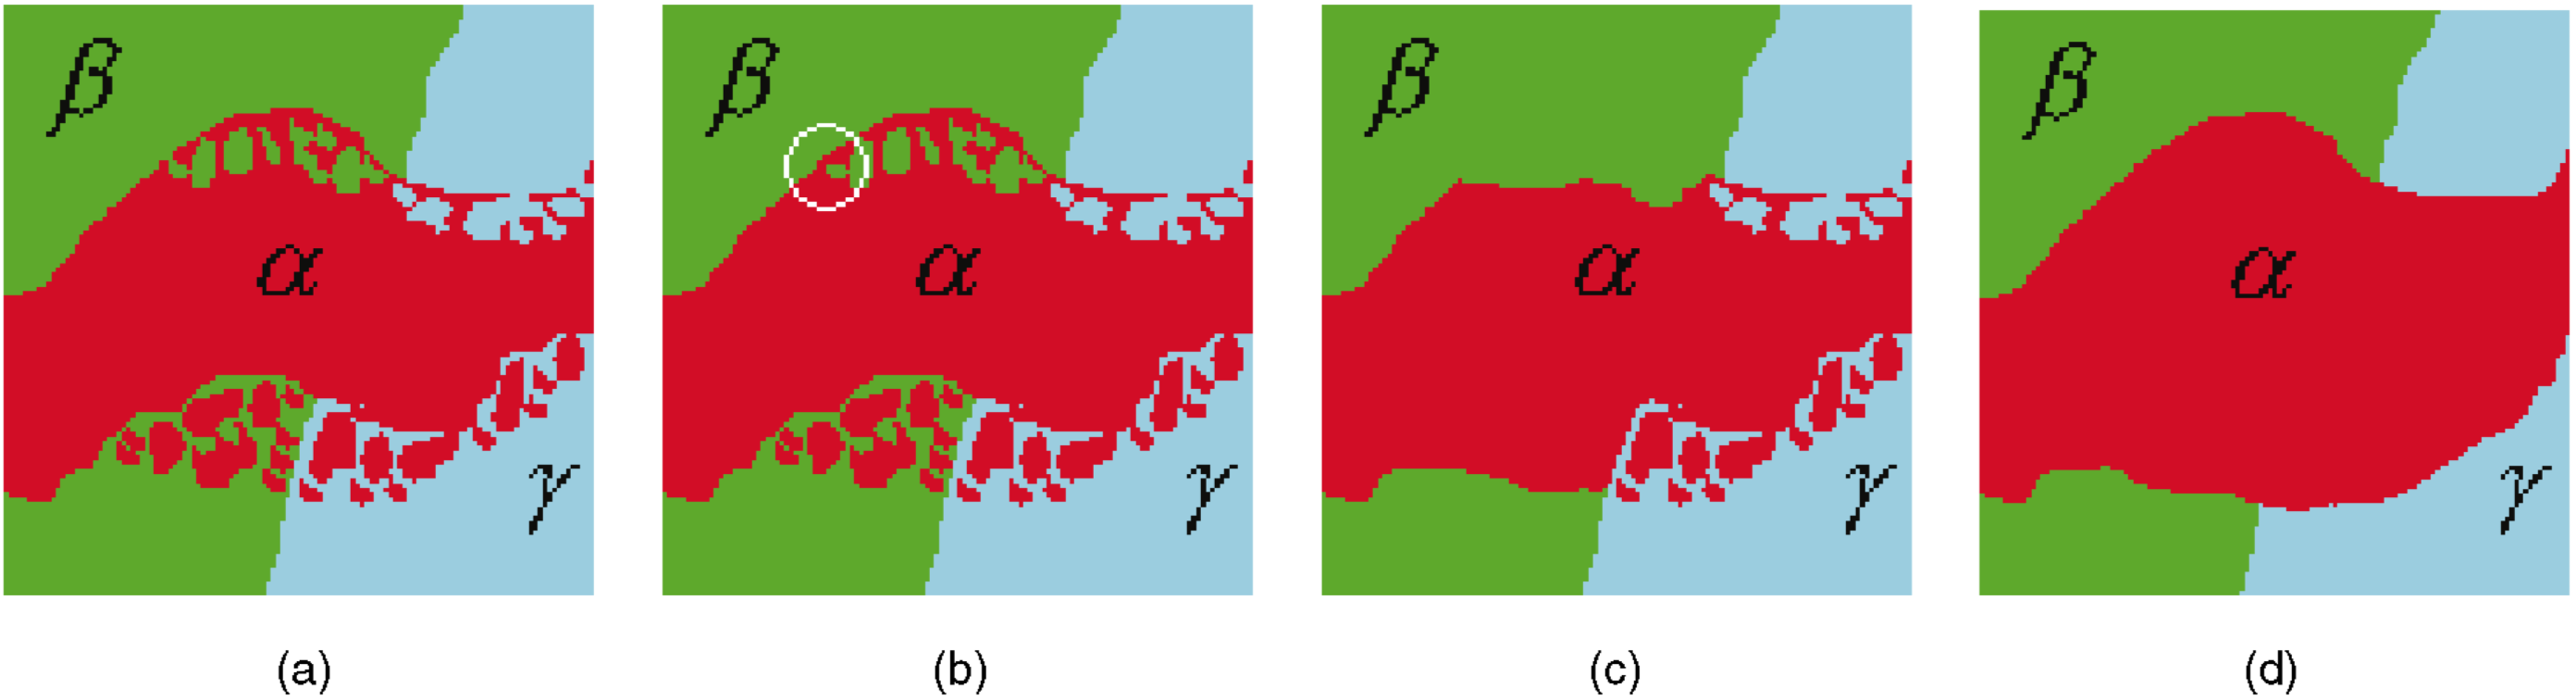
\includegraphics[width=\textwidth]{./operations.png}
\caption{Examples of standard and large moves from a given initial labeling (a). The number of labels is $|L|=3$. A standard moves, (a)$\rightarrow$(b), changes the label of a single pixel(in the circled area). Strong moves, $\alpha - \beta-swap$ (a)$\rightarrow$(c) and $\alpha-expansion$ (a)$\rightarrow$(d), allow large number of pixels to change their labels simultaneously.}
\end{figure}

\begin{description}
\item[Definition] Given a pair of labels $\alpha, \beta$, a move from a partition $P$ to $P^{'}$ is called an $\alpha-\beta-swap$ if $P_l = P_{l}^{'}$ for any label $l \neq \alpha,\beta$. \qed
\item[Definition] Given a label $\alpha$, a move from a partition $P$ to a new partition $P^{'}$ is called an $\alpha-expansion$ if $P_{\alpha} \subset P_{\alpha}^{'}$ and $P_{l}^{'} \subset P_{l}$ for any label $l \neq \alpha$. \qed
\end{description}

Given an input labeling $f$(partition $P$) and a pair of labels $\alpha,\beta$, we wish to find a labeling $\hat{f}$ that minimizes E over all labelings within one $\alpha - \beta$swap of $f$. The following algorithm shows how to minimize such energy function.

\begin{algorithm}
\caption{Algorithm $\alpha - \beta$ Swap}
\begin{algorithmic}[1]
\STATE Start with an arbitrary labeling $f$
\STATE Set success := 0
\FOR{each pair of labels $\{\alpha, \beta\} \subset L$}
\STATE Find $\hat{f} = argminE(f^{'})$ among $f^{'}$ within one $\alpha - \beta$ swap of $f$
\IF{$E(\hat{f}) < E(f)$,}
\STATE Set $f := \hat{f}$ and success := 1
\ENDIF
\ENDFOR
\IF{success == 1}
\STATE Go to 2:
\ENDIF
\end{algorithmic}
\end{algorithm}

To let you understand how an image is modeled into graph, I will give you an example of 1-dimensional image.

\clearpage

\begin{figure}
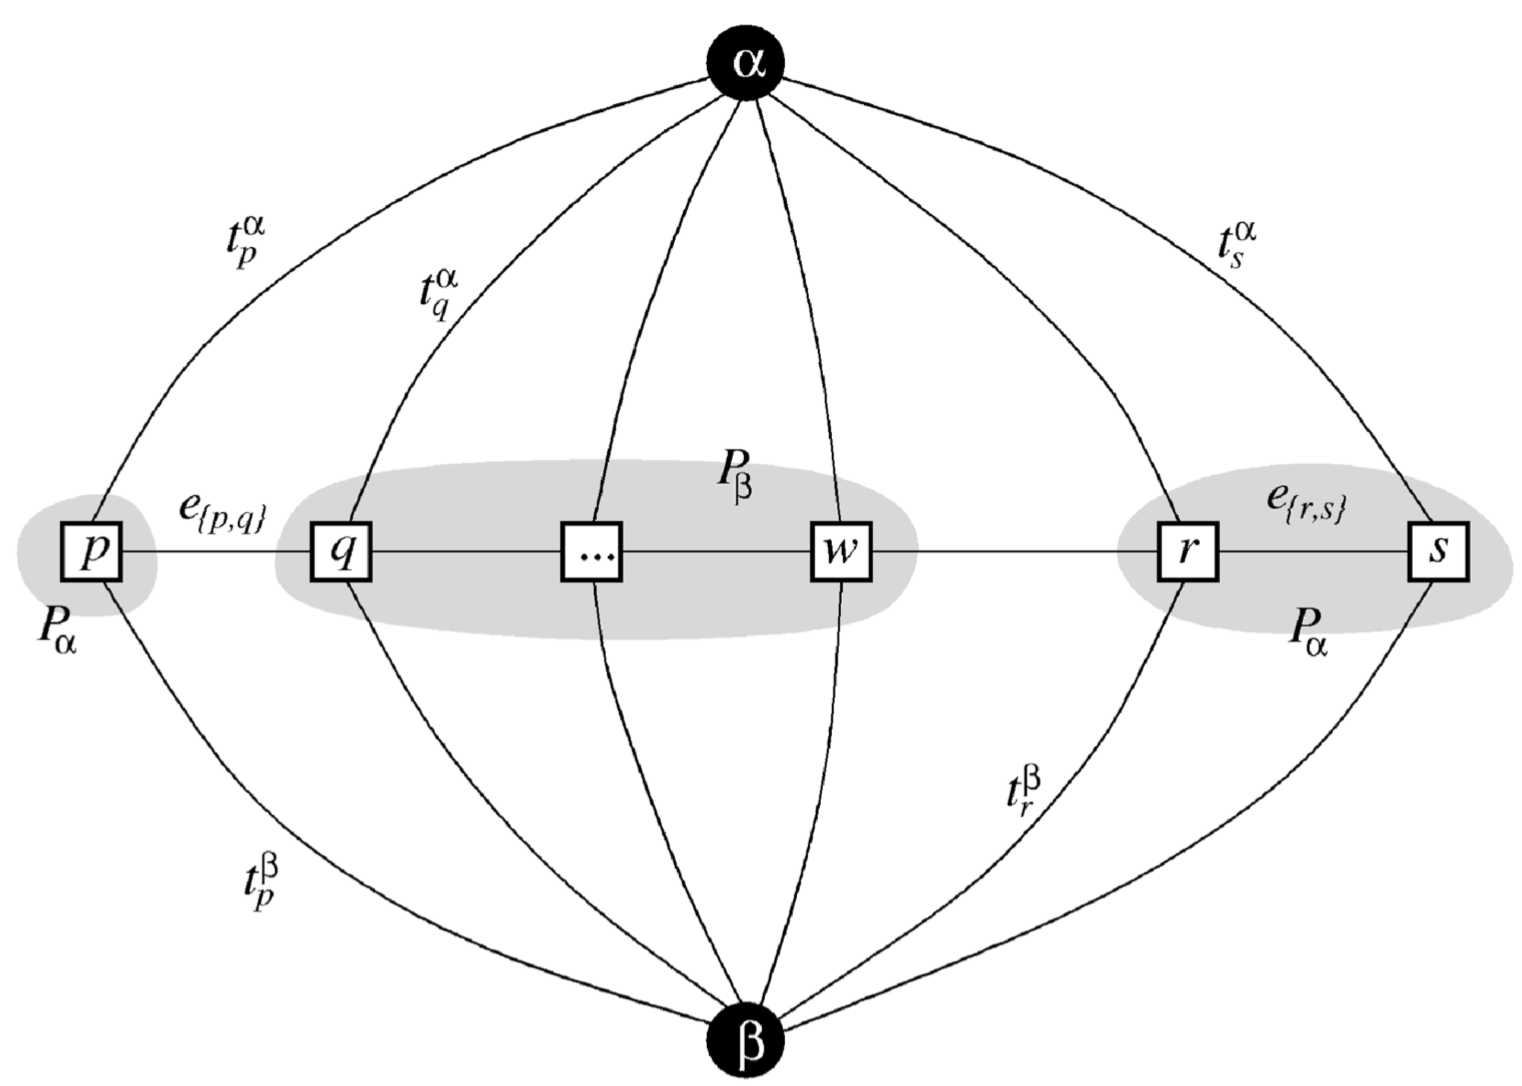
\includegraphics[width=\textwidth]{./graph.png}
\caption{An example of the graph $G_{\alpha\beta}$ for a 1D image. The set of pixels in the image is $P_{\alpha\beta}=P_{\alpha} \cup P_{\beta}$ where $P_{\alpha}=\{p,r,s\}$ and $P_{\beta}=\{q,\cdots,w\}$}
\end{figure}

\begin{table}
\center
\caption{Energy settings for each edge element}
\begin{tabular}{@{}llr@{}} \toprule
Edge & Weight & for\\ \midrule
$t_{p}^{\alpha}$ & $D_p(\alpha) + \sum_{q \in N_p, q \not\in P_{\alpha\beta}}V(\alpha, f_{q})$ & $p \in P_{\alpha\beta}$ \\
$t_{p}^{\beta}$ & $D_{p}(\beta) + \sum_{q \in N_{p}, q \not\in P_{\alpha\beta}}V(\beta, f_{q})$ & $p \in P_{\alpha\beta}$ \\
$e_{p,q}$ & $V(\alpha, \beta)$ & $\{p,q\} \in N, p,q \in P_{\alpha,\beta}$ \\
\end{tabular}
\end{table}
By setting energy like the table above and processing Algorithm 3, we can achieve the goal of the problem. This is because the Ford-Fulkerson gives us the minimum cut of a graph while preserving one-to-one correspondence between pixels and labels. This can be justified by the following theorem.

\begin{description}
\item[Theorem] There is one-to-one correspondence between cuts $C$ on $G_{\alpha\beta}$ and labelings that are one $\alpha - \beta$ swap from $f$. Moreover, the cost of a cut $C$ on $G_{\alpha\beta}$ is $|C|=E(f^{C})$ plus a constant. \qed
\end{description}

 It seems like we can implement the algorithm straightaway. However, we can improve the efficiency of the algorithm 3 by choosing different algorithm in line 4. 
 
 \begin{description}
 \item[Definition] A blocking flow of some network is such a flow that every path from $s$ to $t$ contains at least one edge which is saturated by this flow.
 \item[Definition] A level graph of a network $G$ is a graph built in the following way
\begin{itemize}
\item[1.] For each vertex, we calculate $level[v]$, the shortest path(unweighted) from $s$ to this vertex using only edges with positive capacity. 
\item[2.] We keep only those edges $(u,v)$ for which $level[v] + 1 = level[u]$.
\end{itemize}
Obviously, this network is acyclic.
\end{description}

These definitions come with an important lemma which is crucial in improving algorithm 2.

\begin{description}
\item[lemma] The distances from $s$ to each vertex don't decrease after each iteration, i.e. $level_{i + 1}[v] \geq level_{i}[v]$. \qed
\end{description}

Inspired by the preceding lemma, I now introduce Dinic's Algorithm

\begin{algorithm}
\caption{Dinic's Algorithm}
\begin{algorithmic}[1]
\FOR{each edge $(u,v) \in G$}
\STATE $(u,v).f = 0$
\ENDFOR
\STATE Construct the level graph $G_L$ from a graph $G$
\IF{$level[t] == \infty$}
\STATE Stop and return $f$
\ENDIF
\WHILE{there exists a a path $p$ from $s$ to $t$ in the residual network $G_L$}
\STATE $c_f(p) = min\{c_f(u,v) : (u,v)$ is in $p\}$
\FOR{each edge $(u, v)$ in $p$}
\IF{$(u,v) \in G.E$}
\STATE $(u,v).f = (u,v).f + c_f(p)$
\ELSE
\STATE $(v,u).f = (v.u).f - c_f(p)$
\ENDIF
\ENDFOR
\ENDWHILE
\end{algorithmic}
\end{algorithm}

The algorithm runs in $O(V^{2}E)$ time and is significantly improved compared to naive Ford-Fulkerson which runs in $O(Ef)$.

\chapter{Bayesian Restoration of Images}
\section{The Ising Model}

The restoration of degraded images is a branch of digital picture processing, closely related to image segmentation and boundary finding, and extensively studied for its evident practical importance as well as theoretical interest. In this project, I adopted a Bayesian approach and exploited a hierarchical stochastic model for the original image, based on the \textit{Gibbs distribution}, and a new retoration algorithm, based on stochastic relaxation and \textit{annealing}, for computing the maximum a posteriori(MAP) estimate of the original image given the degraded image.

\begin{description}
\item[Definition] An Ising model is an array of spins (e.g. atoms that can take states $\pm 1$) that are magnetically coupled to each other. If one spin is, say, in the $+1$ state then it is energetically favorable for its immediate neighbours to be in the same state, in the case of \textit{ferromagnetic} model, and in the opposite state, in the case of an \textit{antiferromagnet}.
\end{description}

Let the state $x$ of an Ising model with $N$ spins be a vector in which each component $x_n$ takes values $-1$ or $+1$. If two spins $m$ and $n$ are neighbours we write $(m,n) \in N$. The coupling between neighbouring spins is $J$. The energy of a state $x$ is
$$E(x;J,H) = -\left[\frac{1}{2}\sum_{m,n} J_{mn}x_{m}x_{n} + \sum_{n}Hx_n\right]$$
where $H$ is the applied field. 

At equilibrium at temparature $T$, the probability that the state is $x$ is
$$P(x | \beta, J, H)= \frac{1}{Z(\beta,J,H)} exp[- \beta E(x;J,H)]$$
where $\beta=\frac{1}{\kappa_{B}T}$, $\kappa_{B}$ is Boltzmann's constant, and
$$Z(\beta, J, H) = \sum_{x} exp[-\beta E(x;J,H)]$$

In order to analyze some of the important properties in Ising model, I will introduce a few concepts in Statistical Physics. Consider for example the heat capacity of a system, which is defined to be
$$C = \frac{\partial}{\partial T} \bar{E}$$
where
$$\bar{E} = \frac{1}{Z} \sum_{x} exp(-\beta E(x))E(x)$$
To work out the heat capacity of a system, we might naively guess that we have to increase the temparature and measure the energy change. Heat capacity, however, is intimately related to energy \textit{fluctuations} at constant temparature. Let's start from the partition function,
$$Z = \sum_{x} exp(-\beta E(x))$$
The mean energy is obtained by differentiation with respect to $\beta$:
$$\frac{\partial ln(Z)}{\partial \beta}  = \frac{1}{Z} \sum_{x} -E(x) exp(-\beta E(x)) = -\bar{E}$$
A further differentiation spits out the variance of the energy:
$$\frac{\partial^2 ln(Z)}{\partial \beta^2} = \frac{1}{Z} \sum_{x} E(x)^2 exp(-\beta E(x)) - \bar{E}^2 = <E^2> - \bar{E}^2 = var(E)$$
This result can be interpreted by letting $\lambda = 0$ in a cumulant generating function in a statistical sense.
$$ln\left[E(e^{\lambda E(x)})\right]$$
But the heat capacity is also the derivative of $\bar{E}$ with respect to temparature:
$$\frac{\partial \bar{E}}{\partial T} = -\frac{\partial}{\partial T}\frac{\partial lnZ}{\partial \beta} = -\frac{\partial^2 lnZ}{\partial \beta^2}\frac{\partial \beta}{\partial T} = -var(E)\left(-\frac{1}{\kappa_{B} T^2}\right)$$
So for any system at temparature $T$,
$$C = \frac{var(E)}{\kappa_{B} T^2} = \kappa_{B} \beta^2 var(E)$$
Thus if we can observe the variance of the energy of a system at equilibrium, we can estimate its heat capacity. Notice that when $var(E)$ is constant, that is, a system is at its equilibrium, the heat capacity of the system is inversely proportional to $T^2$.

\section{Monte Carlo simulation}
In this section, I will take an example of two-dimensional planar Ising model and compute its equilibrium using a simple Gibbs-sampling method.  Starting from some initial state, a spin $n$ is selected at random, and the probability that it should be $+1$ given the state of the other spins and the temparature is computed,
$$P(+1 | b_n) = \frac{1}{1 + exp(-2 \beta b_n)}$$
where $\beta = \frac{1}{\kappa_{B} T}$ and $b_n$ is the local field
$$b_n = \sum_{m : (m,n) \in N} J x_m + H$$
After sufficiently many iterations, this procedure converges to the equilibrium distribution. An alternative and computationally friendly form of Gibbs-sampling formula is as follows.\\

$$P(accept; \Delta E, \beta) = \bigg \{ \begin{tabular}{ccc}
$1$ & $\Delta E \leq 0$ \\
$exp(-\beta \Delta E)$ & $\Delta E$ > 0
\end{tabular}$$
where $\Delta E = 2x_nb_n$.

\section{Contrast with Schottky anomaly}

So far, we have dealt with some theories that explains several properties of the Ising model. From now on, I will present an empirical result observed after simulating it in two different settings and show what's the difference between reality and the simulated environment.

A peak in the heat capacity, as a function of temparature, occurs in any system that has a finite number of energy levels; a peak is not in itself evidence of a phase transition. Such peaks were viewed as anomalies in classical thermodynamics, since 'normal' systems with infinite numbers of energy levels have heat capacities that are either constant of increasing function of temparature. In contrast, systems with a finite number of levels produced small blips in the heat capacity graph(Figure 3.1).

Let us refresh our memory of the simplest such system, a two-level system with states $x=0$(energy 0) and $x=1$(energy $\epsilon$). The mean energy is
$$E(\beta) = \epsilon \frac{exp(-\beta \epsilon)}{1 + exp(-\beta \epsilon)} = \epsilon \frac{1}{1 + exp(-\beta \epsilon)}$$
and the derivatives with respect to $\beta$ is
$$\frac{dE}{d\beta} = -\epsilon^2 \frac{exp(\beta \epsilon}{[1 + exp(\beta \epsilon)]^2}$$

\begin{figure}
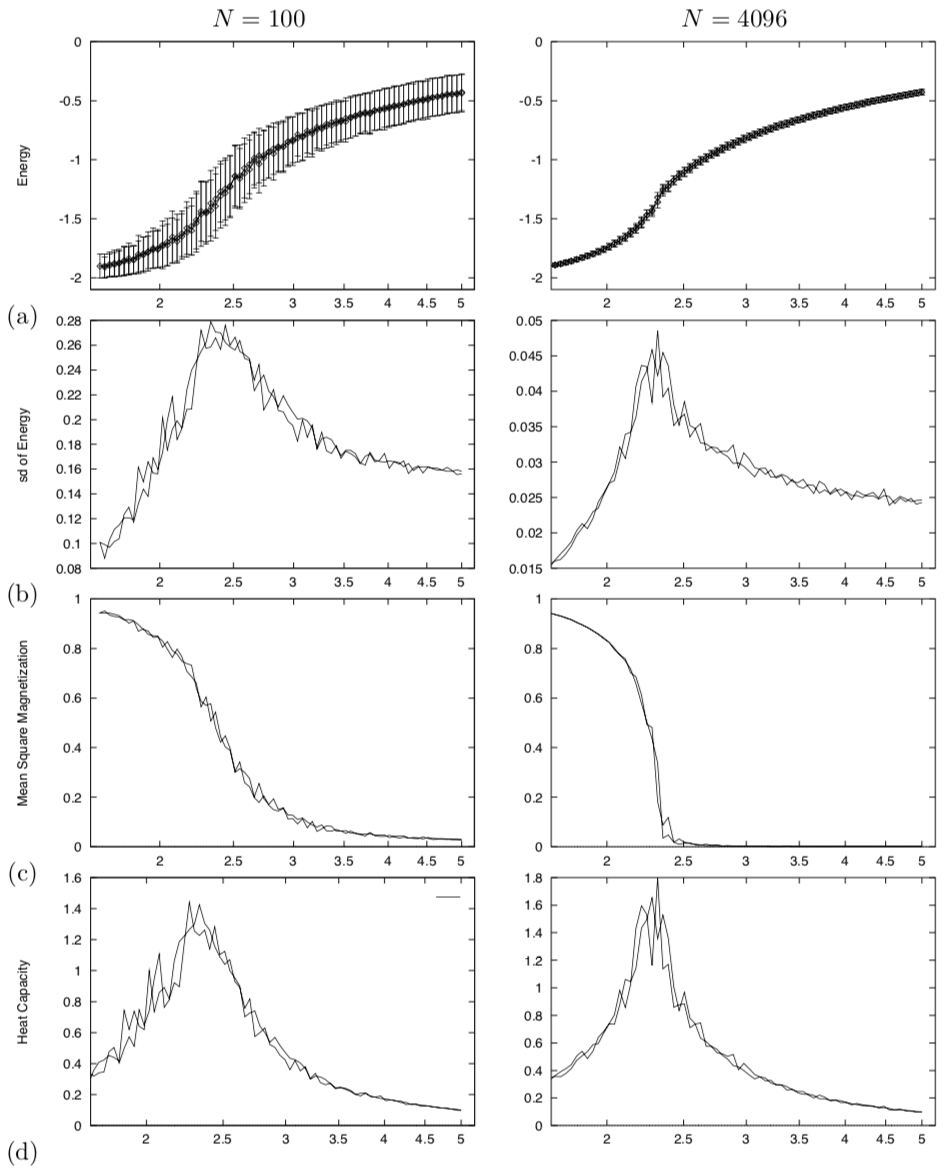
\includegraphics[width=\textwidth]{./Monte.png}
\caption{Detail of Monte Carlo simulations of rectangular Ising Models with $J=1$. (a) Mean energy and fluctuations in energy as a function of temparature. (b) Fluctuations in energy (standard deviation). (c) Mean square magnetization. (d) Heat capacity.}
\end{figure}

So the heat capacity is
$$C = \frac{dE}{dT} = -\frac{dE}{d\beta} \frac{1}{\kappa_{B} T^2} = \frac{\epsilon^2}{\kappa_{B} T^2} \frac{exp(\beta \epsilon)}{[1 + exp(\beta \epsilon)]^2}$$
and the fluctuations in energy are given by $var(E) = C\kappa_{B} T^2 = -\frac{dE}{d\beta}$. 

\begin{figure}
\center
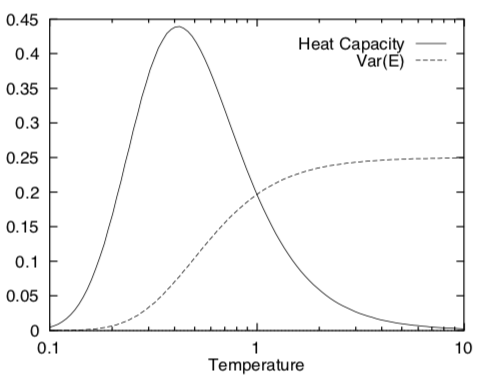
\includegraphics[scale=1]{./Fluc.png}
\caption{Schottky anomaly. Heat capacity and fluctuations in energy as a function of temparature for a two-level system with separation $\epsilon = 1$ and $\kappa_{B} = 1$}
\end{figure}

The heat capacity and fluctuations are plotted in figure 3.2. Notice that there is no peak in their fluctuations; the variance of the energy simply increases monotonically with temparature to a value proportional to the number of independent spins. As a consequence, the heat capacity has a peak around 0.7 and converges to 0 as temparature goes to infinity. 




\end{document}